\documentclass{beamer}
\usepackage{amsmath}
\usepackage{graphicx}
\usetheme{Boadilla}
\usecolortheme{lily}
\setbeamertemplate{footline}
{
  \leavevmode%
  \hbox{%
  \begin{beamercolorbox}[wd=\paperwidth,ht=2.25ex,dp=1ex,right]{author in head/foot}%
    \insertframenumber{} / \inserttotalframenumber\hspace*{2ex} 
  \end{beamercolorbox}}%
  \vskip0pt%
}
\setbeamertemplate{navigation symbols}{}

\title{Question 1-1.5-24}
\author{Teja Vardhan \\ ee24btech11034 }

\date{November 2024}

\begin{document}

\begin{frame}
\titlepage
\end{frame}

\begin{frame}
\frametitle{Problem Statement}
A line intersects the Y-axis and the X-axis at the points \( P(0, b) \) and \( Q(c, 0) \) respectively. If \( (2, -5) \) is the midpoint of \( PQ \), find the coordinates of \( P \) and \( Q \).
\end{frame}

\begin{frame}
\frametitle{Problem Data}
\begin{table}[h]
\centering
\begin{tabular}{|c|c|}
\hline
\textbf{Point} & \textbf{Coordinates} \\ \hline
\( P \) & \( \begin{pmatrix} 0 \\ b \end{pmatrix} \) \\ \hline
\( Q \) & \( \begin{pmatrix} c \\ 0 \end{pmatrix} \) \\ \hline
\( M \) & \( \begin{pmatrix} 2 \\ -5 \end{pmatrix} \) \\ \hline
\end{tabular}
\end{table}
\end{frame}

\section{Solution}
\begin{frame}
\frametitle{Midpoint Formula}
Let the coordinates of points \( P \) and \( Q \) be:
\[
\mathbf{P} = \begin{pmatrix} 0 \\ b \end{pmatrix}, \quad \mathbf{Q} = \begin{pmatrix} c \\ 0 \end{pmatrix}
\]
The midpoint \( M \) is given by:
\[
\mathbf{M} = \begin{pmatrix} 2 \\ -5 \end{pmatrix}
\]
The midpoint formula states:
\[
\mathbf{M} = \frac{1}{2} (\mathbf{P} + \mathbf{Q})
\]
\end{frame}

\begin{frame}
\frametitle{Applying the Midpoint Formula}
Substitute \( \mathbf{P} \), \( \mathbf{Q} \), and \( \mathbf{M} \):
\[
\frac{1}{2} \left(\begin{pmatrix} 0 \\ b \end{pmatrix} + \begin{pmatrix} c \\ 0 \end{pmatrix}\right) = \begin{pmatrix} 2 \\ -5 \end{pmatrix}
\]
Simplify to get:
\[
\frac{1}{2} \begin{pmatrix} c \\ b \end{pmatrix} = \begin{pmatrix} 2 \\ -5 \end{pmatrix}
\]
Multiplying both sides by 2:
\[
\begin{pmatrix} c \\ b \end{pmatrix} = \begin{pmatrix} 4 \\ -10 \end{pmatrix}
\]
\end{frame}

\begin{frame}
\frametitle{Final Answer}
Thus, the coordinates of \( P \) and \( Q \) are:
\[
\mathbf{P} = \begin{pmatrix} 0 \\ -10 \end{pmatrix}, \quad \mathbf{Q} = \begin{pmatrix} 4 \\ 0 \end{pmatrix}
\]
\end{frame}

\begin{frame}
\frametitle{Graphical Representation}
\begin{figure}[h!]
\centering
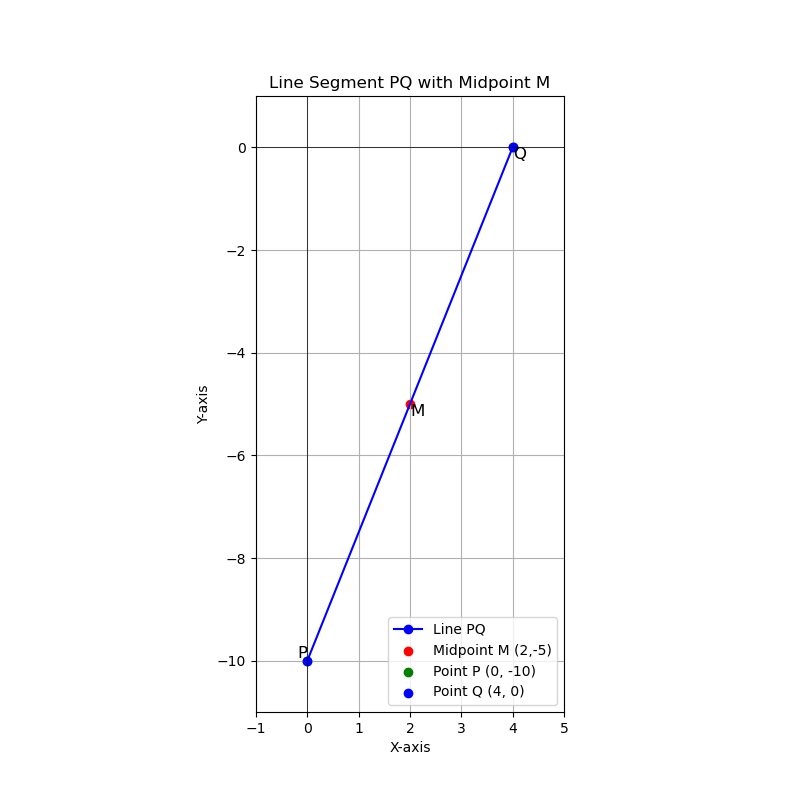
\includegraphics[width=0.7\textwidth]{Figure_1.png}
\caption{Plot showing points \( P \), \( Q \), and midpoint \( M \)}
\label{fig:graph}
\end{figure}
\end{frame}

\end{document}


